\section{Differential Gene Expression Analysis}
This section will discuss the implementation and interpretation of differential gene expression (DGE) analysis using the GEO DataSet mentioned above. The following script creates a DESeqData object from the pre-processed raw count matrix and performs the DGE analysis.
\begin{minted}{R}
# Construct DESeqData object from raw count matrix
dds <- DESeqDataSetFromMatrix(countData=counts_data, colData=coldata, design=~ condition)

# Pre-filtering low-count genes
dds <- dds[rowSums(counts(dds)) >= 1, ]

# Set reference level
dds$condition <- relevel(dds$condition, ref = "control")

# Run Differential Gene Expression analysis
dds <- DESeq(dds)
\end{minted}
Then, the following script unpacks the result of the DEG analysis.
\begin{minted}{R}
# Extract and summarize results
res <- results(dds, contrast = c("condition", "control", "bipolar"), alpha = 0.05)
\end{minted}
The \texttt{results} function calculates log2 fold changes, p-values, and adjusted p-values using the Benjamini-Hochberg method for each gene in the provided read count matrix. The contrast argument specifies the comparison of interest; in this case, we are comparing the Bipolar Disorder (BD) condition to the Control (C) condition based on the \texttt{condition} column. The $\alpha$ argument sets the significance threshold to the widely used value of 0.05, which helps control the false discovery rate (FDR). The resulting object, \texttt{res}, contains the differentially expressed genes and their corresponding statistical measures, which will be further analyzed in the subsequent section of the report.

We conducted two separate experiments to assess the impact of an outlier during the quality control process and subsequent differential expression gene (DEG) analysis. Table \ref{table:unnormalized_summary} summarizes the DESeq2 Differential Gene Expression analysis on the original 36-sample GEO DataSet, identifying 12 significant genes. In contrast, Table \ref{table:normalized_summary} summarizes the DESeq2 Differential Gene Expression analysis on the modified GEO DataSet of 35 samples, excluding the outlier control C\_28. This analysis identified 15 significant genes. The increase in significant genes after removing C\_28 supports the authors' claim in \cite{pacifico2017transcriptome} that this control sample is indeed an outlier, as its removal improved the differentiation between the two cohorts, resulting in a greater number of statistically significant genes for comparison.

\begin{table}[H]
\centering
\begin{minipage}{0.45\textwidth}
\centering
\begin{tabular}{lrr}
\toprule
Category & Count & Percentage \\
\midrule
LFC $>$ 0 (up) & 6 & 0.016\% \\
LFC $<$ 0 (down) & 6 & 0.016\% \\
Outliers & 0 & 0\% \\
Low counts & 12374 & 33\% \\
\bottomrule
\end{tabular}
\caption{DEG of original sample}
\label{table:unnormalized_summary}
\end{minipage}
\hspace{10pt}
\begin{minipage}{0.45\textwidth}
\centering
\begin{tabular}{lrr}
\toprule
Category & Count & Percentage \\
\midrule
LFC $>$ 0 (up) & 5 & 0.013\% \\
LFC $<$ 0 (down) & 10 & 0.027\% \\
Outliers & 0 & 0\% \\
Low counts & 5819 & 16\% \\
\bottomrule
\end{tabular}
\caption{DEG of outlier-normalized sample}
\label{table:normalized_summary}
\end{minipage}
\end{table}


\subsection{Dispersion}
DESeq2 offers a valuable criterion known as dispersion to assess whether its negative binomial model is appropriate for the given GEO data. Dispersion quantifies the extent of variation or spread within the dataset. By default, DESeq2 conducts dispersion analysis using a parameter, denoted as $\alpha$, which satisfies the equation $\sigma^2 = \mu + \alpha \dot \mu^2$. In this equation, $\mu$ represents the mean, and $\sigma^2$ denotes the variance of the sample. Figure \ref{fig:unnormalized_Dispersion} presents the dispersion plot.
\begin{figure}[H]
    \centering
    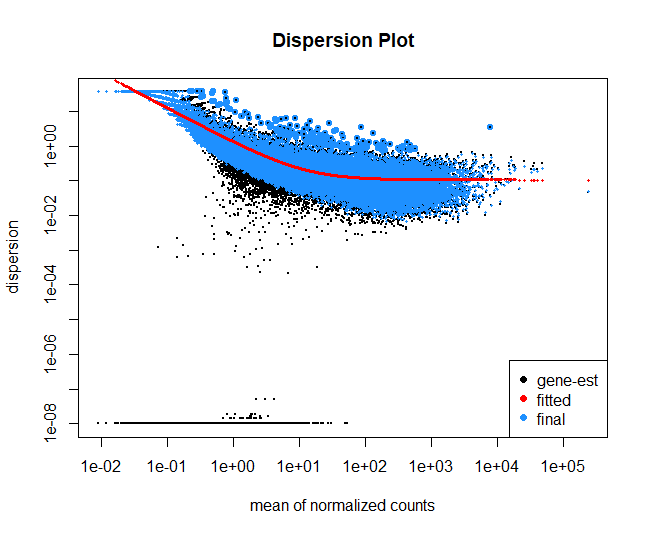
\includegraphics[width=0.4\linewidth]{Plots/DispersionPlot.png}
    \caption{Dispersion Plot}
    \label{fig:unnormalized_Dispersion}
\end{figure}
We can observe that the fitting function is monotonically decreasing. This graph indicates a continuous decrease in dispersion as the mean expression increases. The dispersion estimates generally cluster around the curve, suggesting that the provided GEO DataSet is well-fitted to the DESeq2 model. However, substantial shrinkage is evident due to having only one replicate for each sample in the group.

\subsection{Expression Analysis}
Figure \ref{fig:unnormalized_MA} presents the log fold change MA plot.
\begin{figure}[H]
    \centering
    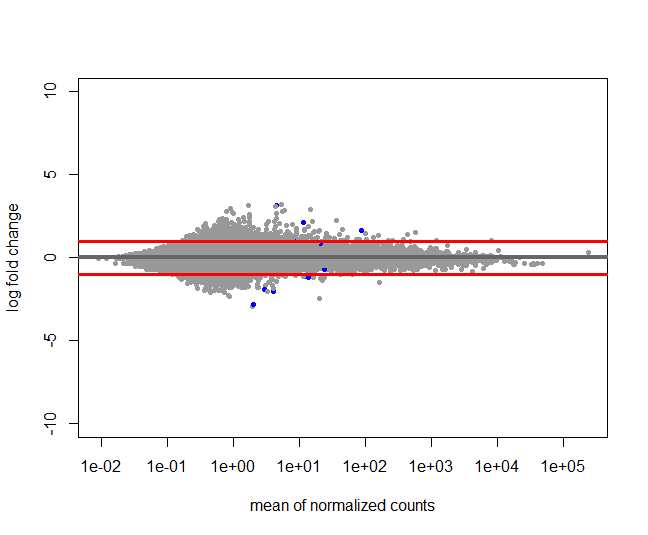
\includegraphics[width=0.4\linewidth]{Plots/MAPlot.png}
    \caption{MA Plot}
    \label{fig:unnormalized_MA}
\end{figure}
This plot visualizes and identifies gene expression changes between two cohorts: "control" and "bipolar" in this case study. The plot displays log fold change (M) on the $y$-axis and the logarithm of the mean normalized gene expression counts for the two conditions on the $x$-axis. 

The plot indicates that genes with lower mean expression values exhibit highly variable log fold changes. The blue dots in Figure \ref{fig:unnormalized_MA} represent differentially expressed genes (DEGs) that have adjusted p-values below the threshold of 0.05. Genes that meet the filtering criteria of a p-value less than 0.05 and a fold change of either greater than 2 (i.e., $\ell>2$) or less than -2 (i.e.,$\ell<-2$) are considered statistically significant. Red vertical lines in the graph mark these thresholds. A fold change greater than 2 (i.e., $\log \ell > 0$) indicates up-regulated genes, while a fold change less than 1 (i.e., $\log \ell < 0$) indicates down-regulated genes. Among the DEGs identified are six up-regulated genes and six down-regulated genes. This analysis is further illustrated in the following plot.
\begin{figure}[H]
    \centering
    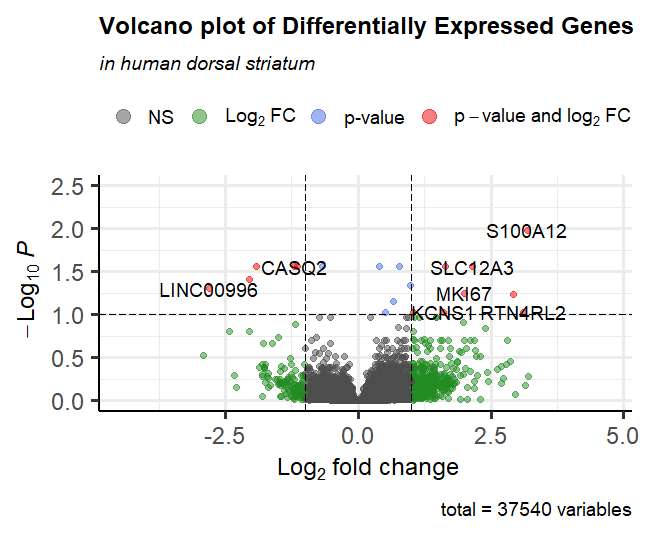
\includegraphics[width=0.5\linewidth]{Plots/VolcanoPlot.png}
    \caption{Volcano plot of DEGs in human dorsal striatum}
    \label{fig:volcano_unnormalized}
\end{figure}
To further analyze the functions of the statistically significant differentially expressed genes, we paired each gene with the reference database provided by the R library \texttt{org.Hs.eg.db}. This library offers mappings between Entrez Gene identifiers and GenBank accession numbers, including Ensemble IDs. Figure \ref{fig:volcano_unnormalized} illustrates the volcano plot of differentially expressed genes. Statistically significant genes are highlighted in red on the plot. Among these, genes with positive log fold changes are considered up-regulated. Table \ref{table:up_regulated} provides a comprehensive list of the up-regulated genes depicted in the volcano plot, along with additional details.
\begin{table}[H]
    \centering
    \begin{tabular}{rrrrrrrrl}
    \toprule
    ENSG ID & baseMean & log2FoldChange & lfcSE & stat & pvalue & padj & symbol \\
    \midrule
    00000070915 & 11.471846 & 2.156212 & 0.487764 & -4.420603 & 9.8426e-06 & 0.0275 & SLC12A3 \\
    00000124134 & 19.494935 & 1.609598 & 0.403496 & -3.989133 & 6.6315e-05 & 0.0927 & KCNS1 \\
    00000148773 & 7.761059 & 2.001743 & 0.478666 & -4.181919 & 2.8905e-05 & 0.0559 & MKI67 \\
    00000163221 & 4.440045 & 3.184795 & 0.629121 & -5.062293 & 4.1424e-07 & 0.0104 & S100A12 \\
    00000165985 & 14.377425 & 2.915072 & 0.700847 & -4.159356 & 3.1914e-05 & 0.0573 & C1QL3 \\
    00000186907 & 4.295899 & 3.110264 & 0.782409 & -3.975241 & 7.0308e-05 & 0.0931 & RTN4RL2 \\
    00000198743 & 1185.410114 & 1.034511 & 0.258776 & -3.997709 & 6.3958e-05 & 0.0927 & SLC5A3 \\
    00000275395 & 87.451458 & 1.643967 & 0.359915 & -4.567649 & 4.9322e-06 & 0.0275 & FCGBP \\
    \bottomrule
    \end{tabular}
    \caption{Complete List of up-regulated genes}
    \label{table:down_regulated}
\end{table}
Some up-regulated genes are associated with immune responses, transmembrane transport, and protein-coding and non-protein-coding functions.

First, SLC12A3, also known as solute carrier family 12 member 3, encodes the sodium-chloride cotransporter (NCC), crucial for sodium and chloride ion reabsorption in the kidney's distal convoluted tubules. The gene’s function in regulating ion homeostasis, cell volume, and neuronal excitability has been well-documented \cite{Zhang2023Role, Li2022Gitelman, Trejo2023CryoEM}. Up-regulation of SLC12A3 is predicted to disrupt these processes, with implications for conditions like Gitelman syndrome \cite{Li2022Gitelman}.

Next, KCNS1, or potassium voltage-gated channel subfamily S member 1, encodes a modulatory subunit that forms heteromultimers with other potassium channels to regulate neuronal excitability and synaptic function. Its up-regulation has been associated with altered synaptic transmission \cite{Koch2020Potassium}. MKI67, a marker for cell proliferation, plays a role in chromosomal organization during mitosis. Up-regulation of MKI67 has been linked to reduced cell division, often serving as a marker for low proliferative activity in cells \cite{Rahman2015Ki67}.

The S100A12 gene encodes calgranulin C, a calcium-binding protein involved in immune response and inflammation. By regulating calcium-dependent processes, including muscle contraction and neuronal signaling, up-regulation may impair immune responses and antibacterial properties \cite{Foell2007S100}.

The role of C1QL3 remains incompletely understood but is linked to immune regulation and inflammation. Similarly, RTN4RL2 is critical for neuronal development and plasticity; its up-regulation correlates strongly with bipolar disorder pathology \cite{Smith2019Neurodevelopment}.

Finally, SLC5A3, encoding a sodium/glucose co-transporter, is essential for glucose uptake and metabolism. Up-regulation impairs glucose metabolism, highlighting its role in cellular energy homeostasis \cite{Chen2019SLC5A}. Lastly, FCGBP, involved in lipid metabolism, remains under explored, though its up-regulation is hypothesized to affect lipid regulation and energy balance \cite{Kim2020Lipids}.

Similarly, the genes exhibiting negative log fold changes are classified as down-regulated. Table \ref{table:down_regulated} provides a complete list of these down-regulated genes, which are represented in the volcano plot, along with additional details.

\begin{table}[H]
    \centering
    \begin{tabular}{rrrrrrrrl}
    \toprule
    ENSG ID & baseMean & log2FoldChange & lfcSE & stat & pvalue & padj & symbol \\
    \midrule
    00000118729 & 13.395064 & -1.199622 & 0.263730 & 4.548668 & 5.3986e-06 & 0.0275 & CASQ2 \\
    00000132744 & 3.952897 & -2.052703 & 0.475144 & 4.320168 & 1.5591e-05 & 0.0392 & ACY3 \\
    00000144681 & 12.769351 & -1.141231 & 0.251624 & 4.535454 & 5.7479e-06 & 0.0275 & STAC \\
    00000239961 & 2.897106 & -1.917298 & 0.431810 & 4.440140 & 8.9900e-06 & 0.0275 & LILRA4 \\
    00000242258 & 2.019025 & -2.799696 & 0.662369 & 4.226795 & 2.3704e-05 & 0.0497 & LINC00996 \\
    \bottomrule
    \end{tabular}
    \caption{Complete list of up-regulated genes}
    \label{table:down_regulated}
\end{table}
Many down-regulated genes are involved in ion transport, cell proliferation, and calcium signaling. 

Firstly, the LILRA4 gene encodes an immunoglobulin-like protein found on the surface of plasmacytoid dendritic cells (pDCs), a rare immune cell subset specialized in antiviral responses and the production of type I interferons \cite{Lim2023LILRA4, Palma2012LILRA4}. Its expression enhances immune regulation, contributing to the innate and adaptive immune response, including during viral infections and inflammatory diseases \cite{Kioon2024LILRA4, Yun2021LILRA4}.

Secondly, the ACY3 gene, also known as aminoacylase 3, encodes a protein critical for deacetylating mercapturic acids in the proximal tubules of the kidney. This gene plays a significant role in maintaining renal function and detoxification processes \cite{Jones2020ACY3}. Additionally, LINC00996, a long intergenic non-coding RNA, has been shown to suppress the migration, invasion, and proliferation of lung adenocarcinoma cells, indicating its role in tumor suppression and cellular homeostasis \cite{Wang2018LINC00996}.

Calsequestrin 2 (CASQ2), a high-capacity calcium-binding protein, functions as an internal calcium reservoir within muscle tissues. It is pivotal in regulating calcium homeostasis, influencing muscle contraction and relaxation cycles \cite{Park2019CASQ2}. Lastly, the STAC gene encodes a scaffold protein that modulates calcium channel expression and function. STAC enhances the activity of calcium channels such as CACNA1H and CACNA1S and slows the inactivation of CACNA1C, which is critical for maintaining cellular calcium signaling \cite{Lopez2021STAC}.

Figure \ref{fig:unnormalized_heatmaps} (a) and (b) illustrate heatmaps depicting sample-to-sample distances and the counts of significant differentially expressed genes (DEGs).
\begin{figure}[H]
    \centering
    \subfloat[\centering Heatmap of pairwise distances among samples]{{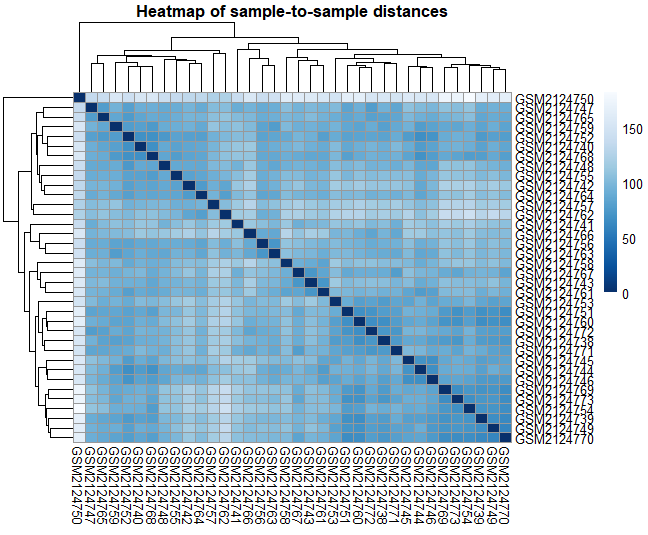
\includegraphics[width=8cm]{Plots/HeatmapPairwisePlot.png} }}%
    \qquad
    \subfloat[\centering Heatmap of significant DEGs]{{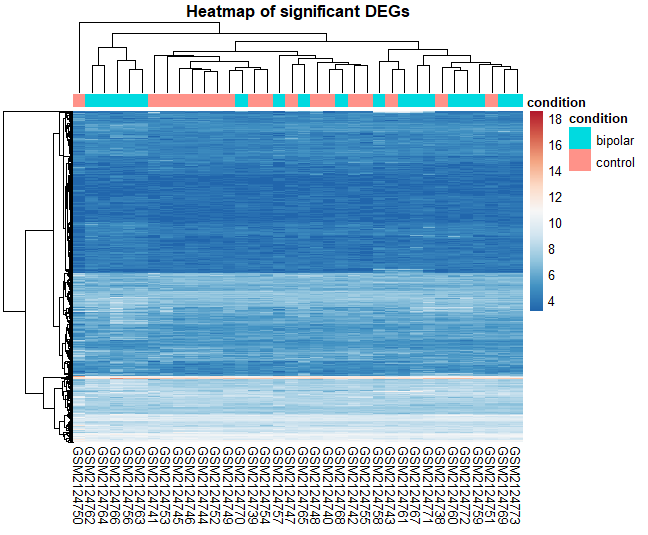
\includegraphics[width=8cm]{Plots/HeatmapDEGPlot.png} }}%
    \caption{Heatmap Plots}
    \label{fig:unnormalized_heatmaps}
\end{figure}
In figure \ref{fig:unnormalized_heatmaps} (a), the correlation heatmap and dendrogram represent all 36 samples based on the Euclidean distances calculated from expression data for all genes. The sample labeled GSM2124750, corresponding to C\_28, was identified as an outlier in the original study \cite{pacifico2017transcriptome}. The heatmap and the dendrogram indicate that it is an outlier. The heatmap aligns with the findings of the original study. Additionally, among the 12 differentially expressed genes identified between groups, some are known immune effectors, with two previously linked to neuropsychiatric disorders.

As a similar study was conducted using the exact same raw sample data, notable differences have emerged in the differentially expressed genes (DEGs) between the two analyses. While our analysis identified several unique DEGs that were not reported in the previous study, there were also genes present in the previous study that are absent from ours.


\begin{table}[H]
    \centering
    \begin{tabular}{llll}
        \toprule
        \text{Ensembl ID}& \text{Gene}& \text{Type of Gene}& \text{Expression Status}\\ 
        \midrule
        00000132744         & ACY3          & Protein-coding        & Under-expressed \\ 
        00000070915         & SLC12A3       & Protein-coding        & Over-expressed  \\ 
        00000124134         & KCNS1         & Protein-coding        & Over-expressed  \\ 
        00000148773         & MKI67         & Protein-coding        & Over-expressed  \\ 
        00000165985         & C1QL3         & Protein-coding        & Over-expressed  \\ 
        00000186907         & RTN4RL2       & Protein-coding        & Over-expressed  \\ 
        00000198743         & SLC5A3        & Protein-coding        & Over-expressed  \\ 
        \bottomrule
    \end{tabular}
    \caption{Genes Absent from Past Study}
    \label{tab:unique_genes}
\end{table}

\begin{table}[H]
    \centering
    \begin{tabular}{llll}
        \toprule
        Ensembl ID          & Gene               & Type of Gene            & Expression Status         \\ 
        \midrule
        ENSG00000253661     & ZFHX4-AS1          & Antisense               & Under-expressed           \\ 
        ENSG00000260912     & RP11-363E7.4       & Sense overlap           & Over-expressed            \\ 
        ENSG00000260064     & RP11-18F14.4       & Sense intronic          & Over-expressed            \\ 
        ENSG00000240032     & RP11-274H2.3       & Antisense               & Over-expressed            \\ 
        ENSG00000219665     & CTD-2006C1.2       & Proc. transcript        & Over-expressed            \\ 
        ENSG00000156219     & ART3               & Protein-coding          & Under-expressed           \\ 
        ENSG00000140853     & NLRC5              & Protein-coding          & Over-expressed            \\ 
        ENSG00000099968     & BCL2L13            & Protein-coding          & Over-expressed            \\ 
        \bottomrule
    \end{tabular}
    \caption{Genes Absent from Our Analysis but Present in Past Study}
    \label{tab:absent_genes}
\end{table}

Some potential factors that may have contributed to the identification of these unique genes include variations in the analytical frameworks used during pipeline development, as well as differences in preprocessing, normalization techniques, and statistical analysis methodologies. Differences in gene annotation databases across studies, particularly in identifying antisense, sense overlap, or protein-coding transcripts, may also explain these variations.


